\section{The Harmonic Oscillator}%- spring and simple pendulum
%As the harmonic oscillator is a very important concept in physics, we want to take a closer look at it. It is used not only to describe sound, but also many other oscillations and vibrations in physics. So the following phenomena can all be described using the harmonic oscillator: a playground swing, a guitar string, a loudspeaker, or a spring with a mass attached to it.
In this chapter, we'll cover the harmonic oscillator. Because of its versatility, it is the physicist's favorite toy model.  
Wherever a system oscillates, it can be approximated to the first order\footnote{That means for reasonably small displacements, it's a ``good'' approximation.} as a harmonic oscillator. This applies for example to a pendulum, a guitar string, and a playground swing.\footnote{Here, the restoring force isn't directly proportional to the displacement, but as an approximation, we can pretend it is --- and get fairly good predictions for the period $T$, for example.}



\begin{comment}
In physics, an oscillation is a periodic variation of a system's state variables over time. Periodic means that after some fixed time $T$, the \textbf{period}, the system's state repeats. For example, picture a swing set at the playground. Its back-and-forth movement is \textit{periodic}.

A prototypical system that exhibits periodic behavior is the harmonic oscillator. Picture a spring hanging down from the ceiling with a mass attached to its bottom half. If you don't touch it, it stays in its so-called \textit{equilibrium state}. Now imagine you pull down the mass a little and then let it go. The mass will move up, through its equilibrium position and then some, slow down, and move down again. It will continue moving up and down, the movement becoming smaller and smaller, until it comes to rest once again in its equilibrium position.

Why does this happen? Well, it takes a force to pull down the spring, because the spring exerts a force pointing back to the equilibrium position. This is what forces the mass to go up when it is below the equilibrium position, and forces it to go down when it is above it. The force always tries to restore the system to its equilibrium state. It is proportional to the distance to its equilibrium position, which is called the \textbf{displacement}.
This proportionality is what makes the oscillator \textit{harmonic}.

The maximum displacement from the equilibrium position is called the \textbf{amplitude}. Interestingly, the \textbf{Period} does not depend on the amplitude! That's one of the things that make the harmonic oscillator special.
A perfect, frictionless harmonic oscillator would keep oscillating forever. When we talk about harmonic oscillators, we'll usually mean this idealized version of it. Reality, of course, is more complicated. The reason a real spring stops swinging after a while is because the system loses energy to the friction with the air and the spring being heated by repeated deformations. 



\textbf{TODO: Text doppelt.} 

Now, what does this have to do with sound waves? For sound, it's the pressure and density of the air that are changing periodically. The restoring force for a specific parcel of air comes, in this case, from interaction with its neighbors. A parcel of higher pressure will try to expand and lower its pressure to the ambient pressure. A parcel of lower pressure will be compressed by its neighboring parcels to get it to ambient pressure. We'll talk about this in more detail later, but as one of my physics professors once said: ``The whole world is made up of harmonic oscillators.'' \footnote{That's a hyperbole, of course, but you'd be surprised how far you can go with this relatively simple model.}
\end{comment}


The most important property of a harmonic oscillator is that the restoring force always points back towards the equilibrium position and becomes stronger the further the object is displaced from it. In equations,
\begin{equation}
    F = - k \cdot x
\end{equation}
where F is the restoring force, $x$ the displacement from the equilibrium position, and $k$ some constant specific to the system. Note how the force has the opposite sign of the displacement --- this way, the force points back to the equilibrium position.

This leads to so-called harmonic oscillations which are described by sine and cosine functions. Why we obtain sine and cosine functions is beyond the scope of this course, since we would need differential equations to explain the derivation. So instead of stepping through the derivations, we'll just give you the solution here:
\begin{align}\label{eq:ho_sol}
   x(t)=A\sin(2\pi ft + \varphi)
\end{align}
Notice how this is very similar to the expression in eq. \ref{eq:shifted_sine}. Let us uncover the meaning of the different quantities.

\begin{description}
\item[Equilibrium position:] The resting position of the object. We have chosen it to be at $x=0$ for convenience. If it were somewhere else, we'd have to add some constant $x_0$ to the right hand side of eq. \ref{eq:ho_sol}.
\item[Amplitude ($A$):] The maximum distance from the equilibrium position.
\item[Frequency ($f$):] The number of oscillations per second.
\item[Period ($T$):] The time needed for one complete oscillation. The period and the frequency are related to each other by $f = 1/T$.
\end{description}
$\varphi$ allows us to let the system start with a different phase, instead of always starting at the equilibrium position.

Now, what does this have to do with sound waves? For sound, it's the pressure and density of the air that are changing periodically. The restoring force for a specific parcel of air comes, in this case, from interaction with its neighbors. A parcel of higher pressure will try to expand and lower its pressure to the ambient pressure. A parcel of lower pressure will be compressed by its neighboring parcels to get it to ambient pressure. We'll talk about this in more detail later.

Let us now explore the two most common and simplest examples of harmonic oscillators. 

\subsection{The spring Pendulum}
\begin{figure}
    \centering
    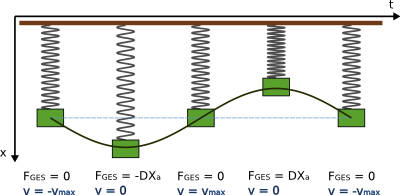
\includegraphics[width=0.5\linewidth]{Bilder/federpendel.png}
    \caption{Spring pendulum}
    \label{fig: Spring_pendulum}
%Quelle : https://lp.uni-goettingen.de/get/text/7976l%
\end{figure}
We attach a mass to a spring. If we pull the mass down and let go, the spring pulls it back towards its equilibrium position.

However, the mass does not stop there. Because of its inertia, it continues moving past the equilibrium position. Inertia is the tendency of an object to resist changes in its motion. An object at rest stays at rest, and a moving object keeps moving unless a force acts on it.

Once the mass has moved past the equilibrium position, the spring pulls it back again. The mass overshoots once more, and the motion repeats, creating a continuous oscillation. \\  
The restoring force is caused by the spring. This force is described by \textbf{Hooke's law}:
\begin{align}
    F =-kx
\end{align}
Where again, $F$ is the restoring force, $x$ is the displacement from the equilibrium position and $k$ is the spring constant. %The minus sign is very important as it tells us that the spring force points always back to equilibrium position. %(Moved to the pervious section)
To describe the oscillation, we need the period $T$ respectively the frequency $f = 1/T$


For a spring oscillator, we can ask questions such as:

\begin{itemize}
    \item Does a larger mass make the oscillation faster or slower?
    \item Does a stiffer spring change the frequency?
    \item Does pulling the spring further (a larger amplitude) affect the frequency?
\end{itemize}


\subsubsection{Experiments}

To investigate which parameters affect the oscillation, we performed the following experiments:

\begin{itemize}
    \item Same spring, different masses
    \item Same spring, different amplitudes
    \item Different springs, same mass
\end{itemize}

To make a fair comparison, we changed only \textbf{one parameter at a time} while keeping all other parameters constant. This allows us to observe how each parameter influences the oscillation.

The experimental results are summarized below.

\subsubsection{Experimental Results}

From our measurements, we found:

\begin{itemize}
    \item The frequency decreases when the mass increases:
    \[
    f \propto \frac{1}{\sqrt{m}}.
    \]

    \item The frequency increases when the spring becomes stiffer:
    \[
    f \propto \sqrt{k}.
    \]

    \item For small oscillations, the frequency is independent of the amplitude. Doubling the amplitude does not change the frequency.
\end{itemize} 

So for the frequency, this leads to: 

\begin{align}
    f = \sqrt{\frac{k}{m}}
\end{align}
\subsection{The Simple Pendulum}

\begin{figure}
    \centering
    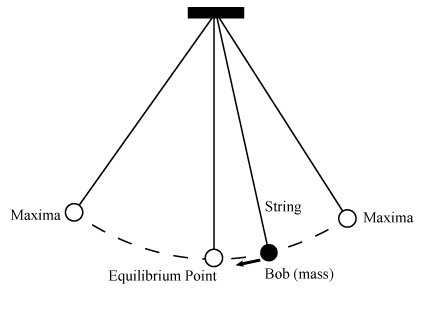
\includegraphics[width=0.4\linewidth]{Bilder/simple_pendulum.png}
    \caption{Simple pendulum}
    \label{fig:simple_pendulum}
    %Quelle; https://www.webassign.net/question_assets/tamucolphysmechl1/lab_1/manual.html %
\end{figure}

A simple pendulum consists of a mass attached to a light string. If we pull the mass to one side and let go, gravity pulls it back towards the equilibrium position.

However, just like the spring oscillator, the mass does not stop there. Because of its inertia, it moves past the equilibrium position. Gravity then pulls it back again, and the motion repeats, creating a continuous oscillation.

For small oscillations, the restoring force is approximately proportional to the displacement. Therefore, a simple pendulum is also a harmonic oscillator.

To describe the oscillation, we again want to determine the period $T$ or the frequency

$
f=\frac{1}{T}.
$

For a simple pendulum, we can ask questions such as:

\begin{itemize}
    \item Does a longer string make the oscillation faster or slower?
    \item Does a heavier mass change the frequency?
    \item Does pulling the pendulum further (a larger amplitude) affect the frequency?
\end{itemize}

\subsubsection{Experiments}

To investigate which parameters affect the oscillation, we performed the following experiments:

\begin{itemize}
    \item Same string length, different masses
    \item Same string length, different amplitudes
    \item Different string lengths, same mass
\end{itemize}

Again, only one parameter was changed at a time while all other parameters were kept constant.

\subsubsection{Experimental Results}

From our measurements, we found:

\begin{itemize}
    \item The frequency decreases when the string becomes longer:
    $
    f \propto \frac{1}{\sqrt{l}}.
    $

    \item The frequency is independent of the mass.
    
    \item For small oscillations, the frequency is independent of the amplitude.
\end{itemize}

The frequency of a simple pendulum is therefore

$
f=\frac{1}{2\pi}\sqrt{\frac{g}{l}},
$

where $g$ is the gravitational acceleration and $l$ is the length of the pendulum.

\subsection{Equation of Motion}

For small oscillations, both systems perform harmonic motion and can therefore be described by a sine or cosine function.

\paragraph{Spring Oscillator}

The position of the mass is given by

\begin{equation}
x(t)=A\sin\left(2\pi\sqrt{\frac{k}{m}}\,t+\varphi\right)
\end{equation}

where

\begin{itemize}
    \item $A$ is the amplitude,
    \item $m$ is the mass,
    \item $k$ is the spring constant,
    \item $\varphi$ is the phase.
\end{itemize}

\begin{figure}[h]
    \centering
    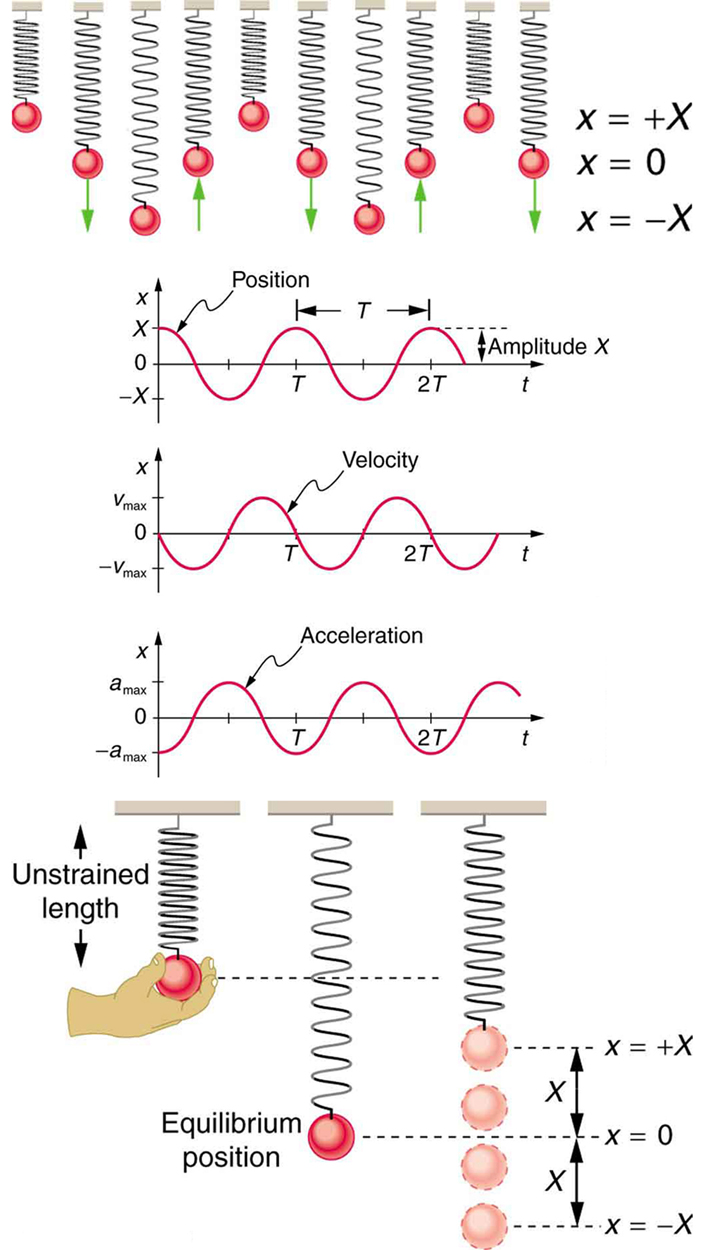
\includegraphics[width=0.7\linewidth]{Bilder/spring_motion.png}
    \caption{Position, velocity and acceleration of a spring oscillator as a function of time.}
    % Quelle: https://openbooks.lib.msu.edu/collegephysics1/chapter/simple-harmonic-motion-a-special-periodic-motion-2/%
    \label{fig:spring_motion}
\end{figure}
The motion of a spring oscillator is shown in Figure \ref{fig:spring_motion}. The graph illustrates the periodic change of the displacement over time. The amplitude corresponds to the maximum displacement from the equilibrium position, while the period is the time required for one complete oscillation.
\paragraph{Simple Pendulum}


For small oscillations, the motion of a simple pendulum is

\begin{equation}
x(t)=A\sin\left(2\pi\sqrt{\frac{g}{l}}\,t+\varphi\right)
\end{equation}

where

\begin{itemize}
    \item $A$ is the amplitude,
    \item $g$ is the gravitational acceleration,
    \item $l$ is the length of the pendulum,
    \item $\varphi$ is the phase.
\end{itemize}

